\chapter{REGULARIZATION METHODS FOR SUBSET ARMA SELECTION}

\section{INTRODUCTION}

Let $\{y_t: t=1,2,\cdots,T\}$ be a sequentially observed discrete and equally-spaced sample from a weakly stationary and homoskedastic process $\{Y_t:t=\cdots,-1,0,1,\cdots\}$. For the purpose of forecasting future realizations i.e. $\hat{y}_{T+h}$ where $h\in\mathbb{N}$, we estimate a model of the general form $y_{t}=f(y_{t-1},y_{t-2},\cdots,y_{t-p},\epsilon_{t-1},\epsilon_{t-2},\cdots,\epsilon_{t-q})+\epsilon_t$. Under homoskedasticitcy, $\{\epsilon_t\}$ is assumed to be white noise with mean 0 and variance $\sigma^2$.  Finite order parameters $p,q\in\mathbb{N}$ quantify the strength past information have on prediction. Define $m=\max\{p,q\}$. In most cases, $m$ is small relative to $T$; however, when cyclical phenomenon is detected, $m\geq S$ where $S$ is the seasonal periodicity. The latter scenario leads to long gaps in relevant information for forecasting.

The seasonal autoregressive moving average (SARMA) process, popularized by \cite{Box1976}, jointly models the temporal short-term and seasonal dynamics of $\{y_t\}$ to forecast future unknown realizations. Let $B$ represent the backshift operator  where $B^ky_{t}=y_{t-k}$ and define polynomial functions $\Phi(B^S)=1-\sum\limits_{J=1}^P \Phi_J B^{SJ}$, $\phi(B)=1-\sum\limits_{j=1}^p \phi_j B^{j}$, $\Theta(B^S)=1+\sum\limits_{K=1}^Q \Theta_K B^{SK}$, and $\theta(B)=1+\sum\limits_{k=1}^q \theta_k B^{K}$. If the seasonal periodicity $S>1$ is known, the SARMA$(p,q)\times(P,Q)_{S}$ process in Equation \ref{eq:sarma} represents a viable family of models for forecasting.
\begin{equation}
\label{eq:sarma}
\Phi(B^S)\phi(B)y_t=\Theta(B^S)\theta(B)\epsilon_t
\end{equation}

The seasonal periodicity $S$ is typically unknown \textit{a priori}. Any SARMA model from Equation \ref{eq:sarma} algebraically reduces to an ARMA$(p^*,q^*)$ process $\phi^*(B)y_t=\theta^*(B)\epsilon_t$ where $\max\{p^*,q^*\}=\max\{PS+p,QS+q\} \textrm{ where } [p,P,q,Q,S]'\in\mathbbm{N}^5$. For example, consider a quarterly SARMA$(1,0)\times(1,0)_{4}$ process $\{x_t\}$ where $\phi_1=0.6$ and $\Phi_1=0.3$. The temporal dynamics of $\{x_t\}$ are equivalently modeled using an ARMA$(5,0)$ process such that $\bm{\phi}=[\phi_1,\phi_2,\phi_3,\phi_4,\phi_5]'=[0.6,0,0,0.3,-0.18]'$ (see Equation \ref{eq:sarma2arma}).
\begin{equation}
\label{eq:sarma2arma}
\begin{split}
\Phi(B^4)\phi(B)x_t&=\epsilon_t\\
(1-0.3B^4)(1-0.6B)x_t&=\epsilon_t\\
(1-0.6B-0.3B^4+0.18B^5)x_t&=\epsilon_t\\
\end{split}
\end{equation}

Fitting an ARMA$(p^*,q^*)$ model to an arbitrary series $\{y_t\}$ requires estimation of AR coefficients $\bm{\phi}=[\phi_1,\cdots,\phi_{p*}]'$ and MA coefficients $\bm{\theta}=[\theta_1,\cdots,\theta_{q^*}]'$. We desire estimates $\hat{\bm{\phi} }$ and $\hat{\bm{\theta} }$ that validate stationary and invertible regulatory assumptions. Stationary and invertible processes guarantee all roots of both characteristic equations, $1-\phi_1z-\phi_2z^2-\cdots -\phi_{p^*}z^{p^*}=0$ and $1+\theta_1z+\theta_2z^2+\cdots +\theta_{q^*}z^{q^*}=0$, are outside the unit circle. Classically, parameter estimation is conducted via method of moments, least squares, or maximum likelihood \citep{Hamilton1994, Cryer2008}. When $q^*=0$, these approaches are simple extensions of linear regression where the set of predictor variables are lagged realizations of the time series. If $q^*>0$, a linear model representation exists, but the presence of MA terms pose an estimation problem since the innovations $\{\epsilon_t\}$ are unobservable and dependent on $\bm{\phi}$ and $\bm{\theta}$. Popular least squares and maximum likelihood estimation methods become far less efficient and require nonlinear optimization techniques.

Any ARMA$(p^*,q^*)$ model that satisfies the invertibility condition has an $AR(\infty)$ representation i.e. $(1-\sum\limits_{j=1}^\infty \phi^\prime_jB^j)y_t=\epsilon_t$. If we know $\bm{\phi}^\prime$, we can obtain the full set $\{\epsilon_t\}$. The residuals $\{\hat{\epsilon}_t: t=\tilde{p}+1,\cdots,T\}$ of a long AR$(p^\prime)$ process fitted to  $\{y_t\}$ can approximate the unobserved $\{\epsilon_t\}$.  This approach was initially proposed by \cite{Hannan1982} to obtain quick estimation of ARMA$(p^*,q^*)$ as it avoids previously mentioned estimation issues. For further information, see \cite{Brockwell2016}.

The model orders $p^*$ and $q^*$ can be heuristically selected through inspection of sample autocorrelation and partial autocorrelation functions (abbreviated ACF and PACF, respectively). This non-scientific approach could lead to misspecified models and possibly poor forecasting performance. Suppose $p$ and $q$ are safe upper bounds such that $p\geq p^*$ and $q\geq q^*$. For the $(p+1)(q+1)$ different ARMA models, final order selection can be based off minimization of some measure of prediction error (PE). Information criteria such as AIC \citep{Akaike1974} or BIC \citep{Schwarz1978} are popular metrics that penalize for model complexity. Stepwise selection algorithms are usually instituted to accelerate this process.

These approaches are best suited for estimating ARMA processes where $\phi_j\neq 0$ and $\theta_k \neq 0$ for $j\in\{1,\cdots,p^*\}$ and $k\in\{1,\cdots,q^*\}$. For the scenario in Equation \ref{eq:sarma2arma}, correct identification of $p^*=5$ and $q^*=0$ still leads to overfitting since truly zero parameters, $\phi_2$ and $\phi_3$, are included in estimation. We define the true process in Equation \ref{eq:sarma2arma} as a subset ARMA$(5,0)$ model where $\bm{\phi}=[\phi_1,\phi_4,\phi_5]'=[0.6,0.3,-0.18]'$. Common approaches for ARMA$(p,q)$ model selection become less efficient and reliable when searching through the $2^{(p+q)}$ unique subset ARMA$(p,q)$ models.	

Let $\bm{y}=[y_{m},\cdots,y_T]'$, $\bm{\epsilon}=[\epsilon_{m},\cdots,\epsilon_T]'$, $\bm{\beta}=[\bm{\phi},\bm{\theta}]'=[\phi_1,\cdots,\phi_p,\theta_1,\cdots,\theta_q]'$, and 
\begin{equation*}
\bm{X}= [\bm{x}'_1,\cdots,\bm{x}'_{p+q}]=	\begin{bmatrix} y_{m-1} & \cdots & y_{m-p} &
					\hat{\epsilon}_{m-1} & \cdots & \hat{\epsilon}_{m-q} \\
					y_{m-2} & \cdots & y_{m-p-1} &
					\hat{\epsilon}_{m-2} & \cdots & \hat{\epsilon}_{m-q-1} \\
					\vdots & \ddots & \vdots &\
					\vdots & \ddots & \vdots & \\
					y_{T-1} & \cdots & y_{T-p} &
					\hat{\epsilon}_{T-1} & \cdots & \hat{\epsilon}_{T-q} \\
	\end{bmatrix},
\end{equation*}
any ARMA$(p,q)$ model can be expressed by $\bm{y}=\bm{X}\bm{\beta}+\bm{\epsilon}$. Recall that $\hat{\epsilon}_t$ are residuals from fitted AR$(p^\prime)$ models used to estimate unknown innovations. Similar to estimation via conditional least squares and conditional maximum likelihood \citep{Hamilton1994}, the first $m-1$ observations are lost in parameter estimation where $m=p^\prime+max\{p,q\}+1$. For reduction of $m$, selection of $p^\prime$ can be based off AIC or BIC  \citep{Hannan1984a,Chen2011}. Also, it is important to note $\{y_t\}$ is assumed to be mean-centered. An additional mean parameter $\mu$ can be included in $\bm{\beta}$ via  binding a column of $1$s to $\bm{X}$.

Presenting the ARMA$(p,q)$ model as a linear Gaussian model is quite advantageous. For both linear and generalized linear models, the lease absolute shrinkage and selection operator (LASSO) of \cite{Tibshirani1996} efficiently combines model selection and estimation. The LASSO estimator in Equation \ref{eq:lasso2} achieves sparsity through $\ell_1$ penalization of the least squares criterion.  The tuning parameter $\lambda >0$ controls overall shrinkage of $\bm{\beta}$ towards 0. Consequentially, the LASSO estimate is a function of $\lambda$, but full solution paths are quickly obtained via well-developed algorithms \citep{Efron2004}. The optimal $\lambda$ is often based off minimization of AIC, BIC, or some generalization of prediction error. The effectiveness of LASSO motivated analogous Bayesian approaches using Laplace priors \citep{Park2008, Yuan2005}. Similarly, hyperpriors placed on $\lambda$ encourage data-driven shrinkage of posterior estimates.
\begin{equation}
\label{eq:lasso2}
\hat{\bm{\beta}}_{L} (\lambda)= \underset{\bm{\beta}}{\textrm{argmin }}  ||\bm{y}-\bm{X}\bm{\beta}||^2 + \lambda \sum\limits_{i=1}^{p+q}|\beta_i|
\end{equation}

Applying LASSO in time series analysis is potentially problematic since the ARMA model matrix $\bm{X}$ contains correlated predictors.  \cite{Nardi2011} explored the consistency properties of $\hat{\bm{\beta}}_{L}$ for AR$(p)$ processes to approximate realizations from ARMA data generating processes. However, high correlation between non-zero and irrelevant ARMA predictors violates an "irrepresentable condition" almost required for sign and model selection consistency \citep{Zhao2006}. \cite{Hebiri2013} demonstrate that highly collinear designs yield underestimation of $\lambda$ and poor prediction. Modified LASSO and other methods with better asymptotic properties mitigate the consequences of correlated predictors.

In our context, $p$ and $q$ should be safely overestimated, resulting in a sparse parameter vector $\bm{\beta}$. In this article, we explore the application of regularization methods to automate subset ARMA$(p,q)$ selection and estimation of $\bm{\beta}$. Section \ref{sec:methods} presents 3 different methods that incorporate subset selection through regularization estimation. The first 2 methods extend off work from \citep{Chen2011}. A discussion of cross-validation techniques explores alternative ways to select regularization tuning parameters. The final regularization method is developed under the Bayesian framework for a contrast to the preceding classical approaches. Section \ref{sec:mc} contains simulation studies evaluating and comparing the different methods. Section \ref{sec:co2app} applies the methods to monthly carbon dioxide time series measured from 2 different atmospheric observatories.










\section{METHODS}
\label{sec:methods}

Assume $y_t$ follows a subset ARMA$(p,q)$ process. Recall the matrix ARMA representation $\bm{y}=\bm{X}\bm{\beta}+\bm{\epsilon}$ where $\bm{\beta}=[\bm{\phi}',\bm{\theta}']=[\beta_1,\cdots,\beta_{p+q}]'$. The set $\mathcal{A}=\{i:\beta_i\neq 0\}$ indicates the AR and MA terms relevant to the true process. If the cardinality $|\mathcal{A}|<p+q$, irrelevant predictors are included in the ARMA model matrix $\bm{X}$. Given observed data $\{y_t: t=m,m+1,\cdots,T\}$, we obtain estimates $\hat{\bm{\beta}}$ for $\bm{\beta}$ and $\hat{\mathcal{A}}=\{i:\hat{\beta}_i\neq 0\}$ for $\mathcal{A}$. Multiple researchers have theoretically explored the asymptotic behavior of penalized estimators including the popular oracle property \citep{Fan2001,Fan2004,Fan2011}. A method for estimating $\bm{\beta}$ is described as oracle if the estimator $\hat{\bm{\beta}}$ asymptotically behaves as an estimator developed under prior knowledge of $\mathcal{A}$. Under these considerations, we describe approaches to estimate ARMA coefficients while simultaneously identifying $\mathcal{A}$ through shrinking irrelevant effects to 0.

\subsection{ADAPTIVE LASSO}

\cite{Zou2006} highlighted the conditional consistency of LASSO and introduced adaptive LASSO (ADLASSO) which enjoys the oracle properties. For a chosen $\eta>0$, we a define vector of weights $\hat{\bm{w}}=|\hat{\bm{\beta}}+1/T|^{-\eta}$ where $\hat{\bm{\beta}}$ represents an initial estimate of $\bm{\beta}$ derived using ordinary least squares (OLS), ridge, or LASSO regression. The additional $1/T$ exists so division by $0$ is prevented. The ADLASSO estimator $\hat{\bm{\beta}}_{AL}$ is described in Equation \ref{eq:adlasso2}. The tuning parameter $\lambda>0$ controls the degree of penalization across all ARMA terms while coefficient-specific weights fine tune shrinkage.
\begin{equation}
\label{eq:adlasso2}
\hat{\bm{\beta}}_{AL} (\lambda)= \underset{\bm{\beta}}{\textrm{argmin }}  ||\bm{y}-\bm{X}\bm{\beta}||^2 + \lambda \sum\limits_{i=1}^{p+q} \hat{w}_{i}|\beta_i|
\end{equation}

For subset ARMA model selection, \cite{Chen2011} showed ADLASSO is an oracle procedure under 3 regulatory assumptions when $\hat{\bm{\beta}}=(\bm{X}'\bm{X})^{-1}\bm{X}'\bm{y}$. Proof of this result followed from using a long AR$(p^\prime)$ process to estimate unknown innovations. Simulation results indicated best empirical performance when the initial estimate $\hat{\bm{\beta}}=\hat{\bm{\beta}}_L$. Following from \cite{Zou2006} and \cite{Chen2011}, we fix $\eta=2$ and only consider $\hat{\bm{\beta}}_L$ in the formulation of $\hat{\bm{w}}$.

\subsection{ADAPTIVE ELASTIC NET}


\subsection{OPTIONS FOR SELECTING TUNING PARAMETERS}
Let $\mathcal{M}_1$ and $\mathcal{M}_2$ represent two competing subset ARMA($p$,$q$) models

Penalized estimation via ENET of autoregressive parameters $\hat{\bm{\phi}}_{\lambda,\alpha}$ and $\hat{\bm{\theta}}_{\lambda,\alpha}$ using LASSO or ENET are dependent on selection of tuning parameters $\lambda$ and  $\alpha$.

\cite{Bergmeir2018} performs a simulation study to examine the validity of using different model selection procedures to estimate predictive performance. From the literature, 

\subsubsection{SELECTION BASED ON AIC OR BIC}

\subsubsection{SELECTION BASED ON OOS FORECAST EVALUATION}

\begin{figure}[htbp!]
	\caption{Variations of Out-of-Sample Procedures for Model Selection}
	\label{fig:oosplots}
	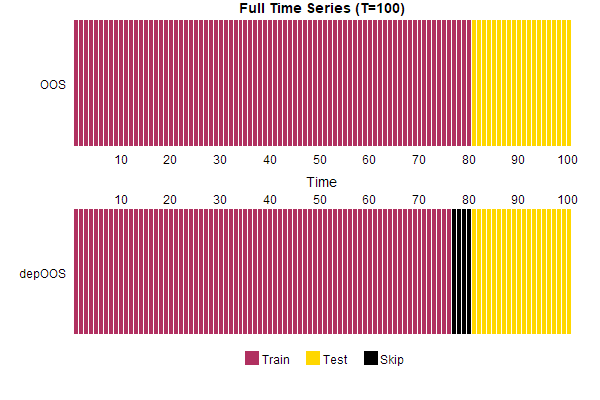
\includegraphics[scale=0.7]{oosplots}
\end{figure}

\subsubsection{SELECTION BASED ON CV FOR INDEPENDENT DATA}

\begin{figure}[htbp!]
	\caption{General $K$-fold Cross-Validation for Model Selection for $K=5$ (top) and $K=10$ (bottom)}
	\label{fig:kcvplots}
	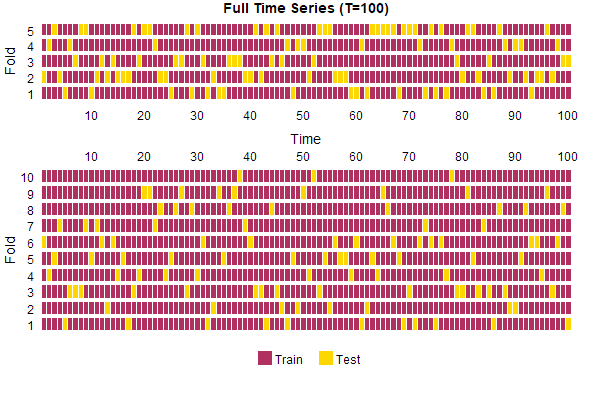
\includegraphics[scale=0.7]{kcvplots}
\end{figure}

\subsubsection{SELECTION BASED ON CV FOR DEPENDENT DATA}

\begin{figure}[htbp!]
	\caption{Non-Dependent $K$-fold Cross-Validation for Model Selection for $K=5$ (top) and $K=10$ (bottom)}
	\label{fig:depkcvplots}
	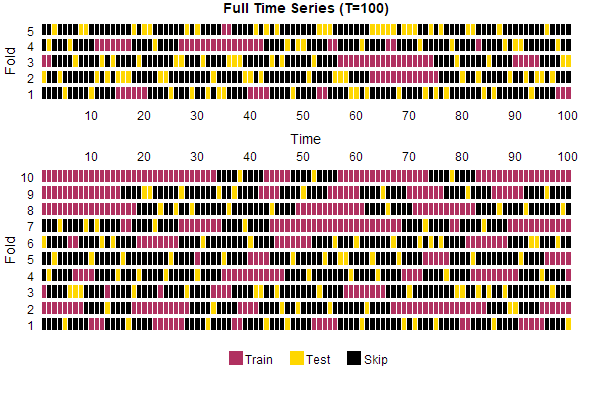
\includegraphics[scale=0.7]{depkcvplots}
\end{figure}

\begin{figure}[htbp!]
	\caption{Non-Dependent $K$-Block Cross-Validation for Model Selection for $K=5$ (top) and $K=10$ (bottom)}
	\label{fig:bcvplots}
	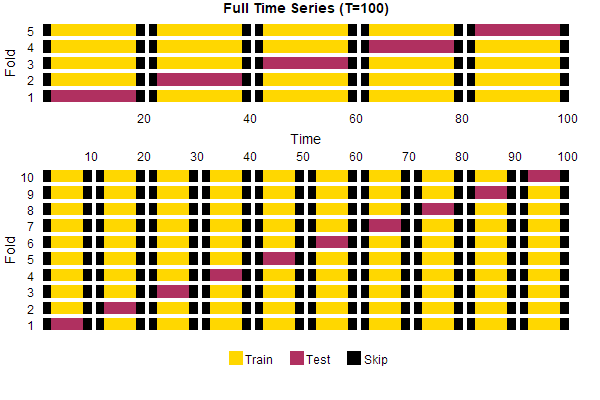
\includegraphics[scale=0.7]{bcvplots}
\end{figure}

\begin{figure}[htbp!]
	\caption{Leave-One-Block-Out Cross-Validation for Model Selection}
	\label{fig:lobocvplots}
	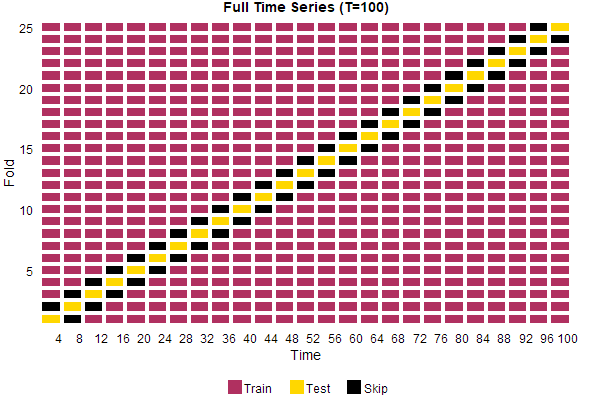
\includegraphics[scale=0.7]{lobocvplots}
\end{figure}

In the time series context, the best model minimizes forecasting error for future observations  unrealized during the model building  

\subsection{BAYESIAN PREDICTIVE POSTERIOR PROJECTION METHOD}
The classic method for model selection within the Bayesian framework begins with a reparameterization of the AR and MA coefficients to $\phi_i^*=\phi_i$ and $\theta_j^*=\theta_j$.

Since the introduction of Bayesian LASSO, research in Bayesian regularization methods has exploded over the last ten years. Bayesian methods analogous to adaptive lasso \citep{Leng2014}, elastic net \citep{Li2010a}, and adaptive elastic net \citep{Stankiewicz2015} have been introduced and applied. \cite{Polson2010}





\section{MONTE CARLO SIMULATIONS}
\label{sec:mc}
Multiple Monte Carlo studies are performed to evaluate and compare ADLASSO, ADENET, and BPP on subset ARMA selection. Consider the three time series $\{y_{1,t}\}$, $\{y_{2,t}\}$, and $\{y_{3,t}\}$ generated by the Gaussian ARMA processes expressed in Equations \ref{eq:simarma1}, \ref{eq:simarma2}, and \ref{eq:simarma3} and abbreviated Models I, II, and III, respectively.
\begin{equation}
	\label{eq:simarma1}
	y_{1,t}=0.8y_{1,t-1}+0.7y_{1,t-6}-0.56y_{1,t-7}+\epsilon_{1,t}
\end{equation}
\begin{equation}
	\begin{split}
	\label{eq:simarma2}
	y_{2,t}&=0.8y_{2,t-1}+0.7y_{2,t-6}-0.56y_{2,t-7}\\
	&+0.8\epsilon_{2,t-1}+0.7\epsilon_{2,t-6}+0.56\epsilon_{2,t-7}+\epsilon_{2,t}
	\end{split}
\end{equation}
\begin{equation}
	\label{eq:simarma3}
	y_{3,t}=0.8\epsilon_{3,t-1}+0.7\epsilon_{3,t-6}+0.56\epsilon_{3,t-7}+\epsilon_{3,t}
\end{equation}
The errors $\{\epsilon_{1,t}\}$, $\{\epsilon_{2,t}\}$, and $\{\epsilon_{3,t}\}$ are i.i.d. Gaussian processes with $0$ mean and variance $\sigma^2$. Models I, II, and III are algebraically equivalent to the first three SARMA$(p,q)\times(P,Q)_6$ models found in \cite{Chen2011}, and similarly, we generate samples from these models of length $T\in \{120, 240, 360\}$ in our Monte Carlo experiments. Furthermore, we consider different choices for $\sigma\in\{0.5,1,1.5\}$ to explore sensitivity to noise. 

The proxy innovations $\{\hat{\epsilon}_{k,t}\}$ are obtained from long AR$(p^\prime)$ models where $p^\prime=10\log_{10}(T)$. Contrary to \cite{Chen2011}, better performance was observed when $p^\prime$ is fixed versus model selection via AIC. Estimation of $\bm{\phi}^\prime$ is obtained from Yule-Walker equations for ADLASSO and ADENET, and from Bayesian linear regression for BPP.

Results from both frequentist approaches heavily depend on the estimated weights $\hat{\bm{w}}=(|\tilde{\bm{\beta}}|+1/T)^{-\eta}$. Suggested by \cite{Zou2006} and used in \cite{Chen2011}, we only consider $\eta=2$. Specifically for ADLASSO, best empirical performance across all experiments occurred when $\tilde{\bm{\beta}}=\tilde{\bm{\beta}}_{LASSO}$ \citep{Chen2011}; therefore, we do not consider LS and RIDGE based weights in our study. In regards to ADENET, we experiment with both ENET and LASSO estimated $\tilde{\bm{\beta}}$.





\section{APPLICATION}
\label{sec:co2app}
Carbon dioxide $\textrm{CO}_2$ levels are constantly measured at strategically placed atmospheric monitoring observatories around the world to track climate change. The {\bf datasets} package in {\bf R} \citep{RCORETEAM} contains a monthly time series of  $\textrm{CO}_2$ levels for January 1959 to December 1997 measured in Mauna Loa, Hawaii, United States. The {\bf TSA} package in {\bf R} \citep{RTSA} contains a similar but shorter series  measured  in Alert, Nunavut, Canada, from January 1994 to December 2004. Let $\{x_{1,t}:t=1,2,\cdots,468\}$ represent the Mauna Loa data, and $\{x_{2,t}:t=1,2,\cdots,132\}$ represent the Alert data. Both $\{x_{1,t}\}$ and $\{x_{2,t}\}$ are nonstationary in mean and cyclical with seasonal periodicity $S=12$. The latter series $\{x_{2,t}\}$ serves as a primary textbook example  to demonstrate the selection, fitting, and forecasting of seasonal models \citep{Cryer2008}. Following the examples provided in \cite{Cryer2008,Chen2011}, subset SARMA$(p,q)\times(P,Q)_{12}$ models utilized at both locations are applied after seasonal and regular differencing . 

Define $y_{k,t}=\Delta_1\Delta_{12}x_{k,t}$ for $k\in\{1,2\}$  where $\Delta_s$ is the difference operator such that $\Delta_s y_t=y_t-y_{t-s}$.  Using all variations of adaptive lasso, adaptive elastic net, and projection model selection, we fit subset ARMA($14,14$) models to $\{y_{1,t}:t=1,2,\cdots,372\}$ corresponding to data prior to 1990 and $\{y_{2,t}:t=1,2,\cdots,108\}$ corresponding to data prior to 2003. The remaining portions $\{y_{1,t}:t=373,374,\cdots,468\}$ and $\{y_{2,t}:t=109,110,\cdots,132\}$ are intentionally preserved for forecasting comparison. Figures \ref{fig:co2plots} and \ref{fig:co2plots2} illustrate the division of the data into fitting and forecasting periods, as well as, the progression of seasonal and regular differencing for Mauna Loa and Alert, respectively.

\begin{figure}[htbp!]
	\centering
	\caption{Plots of $x_{1,t}$ (Top),$\Delta_{12}x_{1,t}$ (Middle), and $\Delta_1\Delta_{12}x_{1,t}$ (Bottom) Partitioned Into Fitting (solid) and Forecasting (dotted) Periods}
	\label{fig:co2plots}
	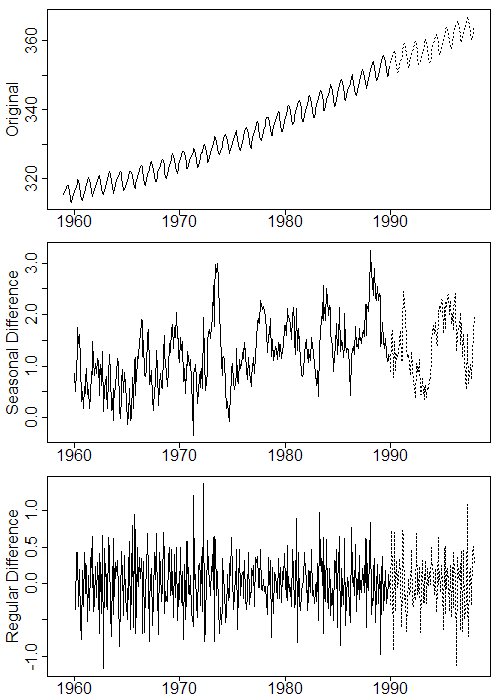
\includegraphics[scale=0.8]{co2plots}
\end{figure}

\begin{figure}[htbp!]
	\centering
	\caption{Plots of $x_{2,t}$ (Top),$\Delta_{12}x_{2,t}$ (Middle), and $\Delta_1\Delta_{12}x_{2,t}$ (Bottom) Partitioned Into Fitting (solid) and Forecasting (dotted) Periods}
	\label{fig:co2plots2}
	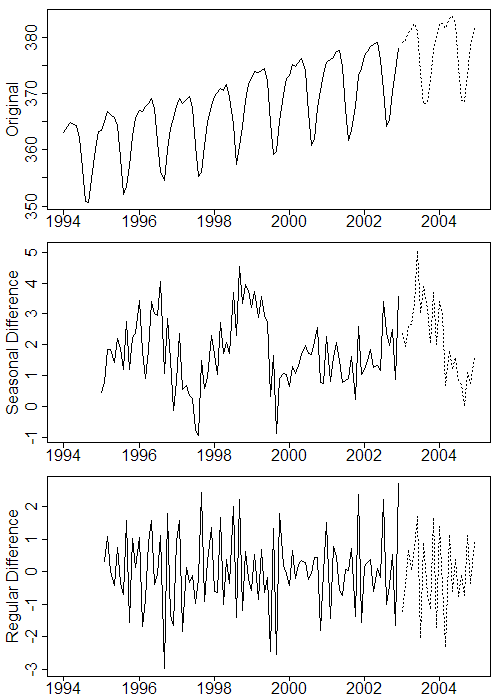
\includegraphics[scale=0.8]{co2plots2}
\end{figure}


The DGPs of $\{y_{1,t}\}$ and $\{y_{2,t}\}$ are hidden to the observer; therefore, evaluating the ability of a subset selection method to uncover the truth is an impossible task. The exploration into various cross-validation methods was motivated by the terminal desire to produce forecasts. Using the final subset ARMA($14,14$) models selected from the full library of methods presented in this paper, we obtain rolling $1$-step ahead predictions $\hat{y}_{k,t}$ over the full forecasting period of length $n_k$ where $k\in\{1,2\}$. As previously determined, $n_1=96$ and $n_2=24$.  Methods are evaluated based on root mean squared error (RMSE), mean absolute percentage error (MAPE), mean bias (MB), and mean directional bias (MDB). The formulas for these metrics are expressed in Equation \ref{eq:fmetrics}. In the expression for MDB, $\textrm{sgn}(x_t)=1$ if $x_t>0$ and $\textrm{sgn}(x_t)=-1$ if $x_t<0$.

\begin{equation}
\label{eq:fmetrics}
\begin{split}
	RMSE_k&=\frac{1}{n_k} \sum\limits_{j=1}^{n_k} (y_k-\hat{y}_k)^2 \\
	MAPE_k&=\frac{100}{n_k} \sum\limits_{j=1}^{n_k} \bigg|\frac{y_{k,j}-\hat{y}_{k,j}}{y_{k,j}}\bigg| \\
	MB_k&=\frac{1}{n_k} \sum\limits_{j=1}^{n_k} (y_{k,j}-\hat{y}_{k,j}) \\
	MDB_k&=\frac{1}{n_k} \sum\limits_{j=1}^{n_k} \textrm{sgn}(y_{k,j}-\hat{y}_{k,j})\\
\end{split}
\end{equation}






\section{CONCLUSION}
